\documentclass[review]{elsarticle}

\usepackage{lineno,hyperref}
\usepackage{arydshln}
\usepackage{glossaries}
\modulolinenumbers[5]
\newglossaryentry{demN}{name=747,description=The total number of respondents in the dataset}
\newglossaryentry{demfemale}{name=76.44,description=The share of female respondents in the dataset}
\newglossaryentry{demmale}{name=23.56,description=The share of male respondents in the dataset}
\newglossaryentry{struggling}{name=5.89,description=The share of respondents who struggle financially}

\journal{Journal of \LaTeX\ Templates}

%%%%%%%%%%%%%%%%%%%%%%%
%% Elsevier bibliography styles
%%%%%%%%%%%%%%%%%%%%%%%
%% To change the style, put a % in front of the second line of the current style and
%% remove the % from the second line of the style you would like to use.
%%%%%%%%%%%%%%%%%%%%%%%

%% Numbered
%\bibliographystyle{model1-num-names}

%% Numbered without titles
%\bibliographystyle{model1a-num-names}

%% Harvard
%\bibliographystyle{model2-names.bst}\biboptions{authoryear}

%% Vancouver numbered
%\usepackage{numcompress}\bibliographystyle{model3-num-names}

%% Vancouver name/year
%\usepackage{numcompress}\bibliographystyle{model4-names}\biboptions{authoryear}

%% APA style
%\bibliographystyle{model5-names}\biboptions{authoryear}

%% AMA style
%\usepackage{numcompress}\bibliographystyle{model6-num-names}

%% `Elsevier LaTeX' style
\bibliographystyle{elsarticle-num}
%%%%%%%%%%%%%%%%%%%%%%%

\begin{document}

\begin{frontmatter}

\title{Sustainable clothing in youngsters \tnoteref{mytitlenote}}
%\tnotetext[mytitlenote]{Fully documented templates are available in the elsarticle package on \href{http://www.ctan.org/tex-archive/macros/latex/contrib/elsarticle}{CTAN}.}

%% Group authors per affiliation:
\author[]{Sandra Rousseau\corref{mycorrespondingauthor}}
%\address{Radarweg 29, Amsterdam}
\cortext[mycorrespondingauthor]{Corresponding author}
\ead{sandra.rousseau@kuleuven.be}
%% or include affiliations in footnotes:
\author[mymainaddress]{Ra\"{i}sa Carmen}




\address[mymainaddress]{CEDON, KU Leuven}
%\address[mysecondaryaddress]{}

\begin{abstract}
This article investigates how important sustainability is for youngsters when buying clothing. The focus group are respondents between 15 and 35 years old in Flanders and Brussels (Belgium).
\end{abstract}

\begin{keyword}
Discrete choice model\sep sustainable clothing \sep choice modelling \sep stated choice
\end{keyword}

\end{frontmatter}

\linenumbers

\section{Introduction}\label{sec:Intro}
This article discusses the results of a survey on sustainable consumption of clothing/fashion with youngsters in the Flemish and the Brussels-Capital Regions (Belgium).

Negative environmental and social are associated with the production, usage, maintenance, and disposal of clothes \citep{Roos2016}. Figure~\ref{fig:MaterialFlow} summarizes the current, problematic global material flow. The most common fibers used for clothes are synthetic (mostly coal- and petroleum-based) and cotton. As synthetic fibers are usually non-renewable and traditional cotton-growing uses excessive amounts of water, pesticides, and fertilizers, the industry if actively searching for alternatives \citep{Meyer}. Hazardous chemicals are used to turn the raw materials into clothing and textiles \citep{VanDerVelden,Kant2012}. Next, the clothes may have to be transported over a long distance to get to the consumer. During the use and maintenance phase, washing the clothes requires water and electricity, the detergents may be hazardous to the environment, and synthetic fibers may release micro-fibers which is a real threat to marine environments \citep{Cesa2017,DeFalco2018, Thevenon}. Lastly, there are major ethical concerns about the way the clothing industry is set up. Scandals about child labor, low wages, abuse, and accidents (like the one in Rana Plaza in 2013) are rampant and the Belgian government is lagging behind when it comes to forcing industry to take responsibility\citep{Goethals2018}. Unfortunately, \cite{Morlet2017} show that clothes sales doubled from 50 to 100 billion units per year between 2000 and 2015. It is therefor no surprise that textiles and fashion are currently on the agenda of, for instance, WRAP in the UK \citep{WrapUK}, ECAP in Europe \citep{ECAP} and the Ellen MacArthur Foundation \citep{Morlet2017}. 
\begin{figure}[ht]
\begin{center}
 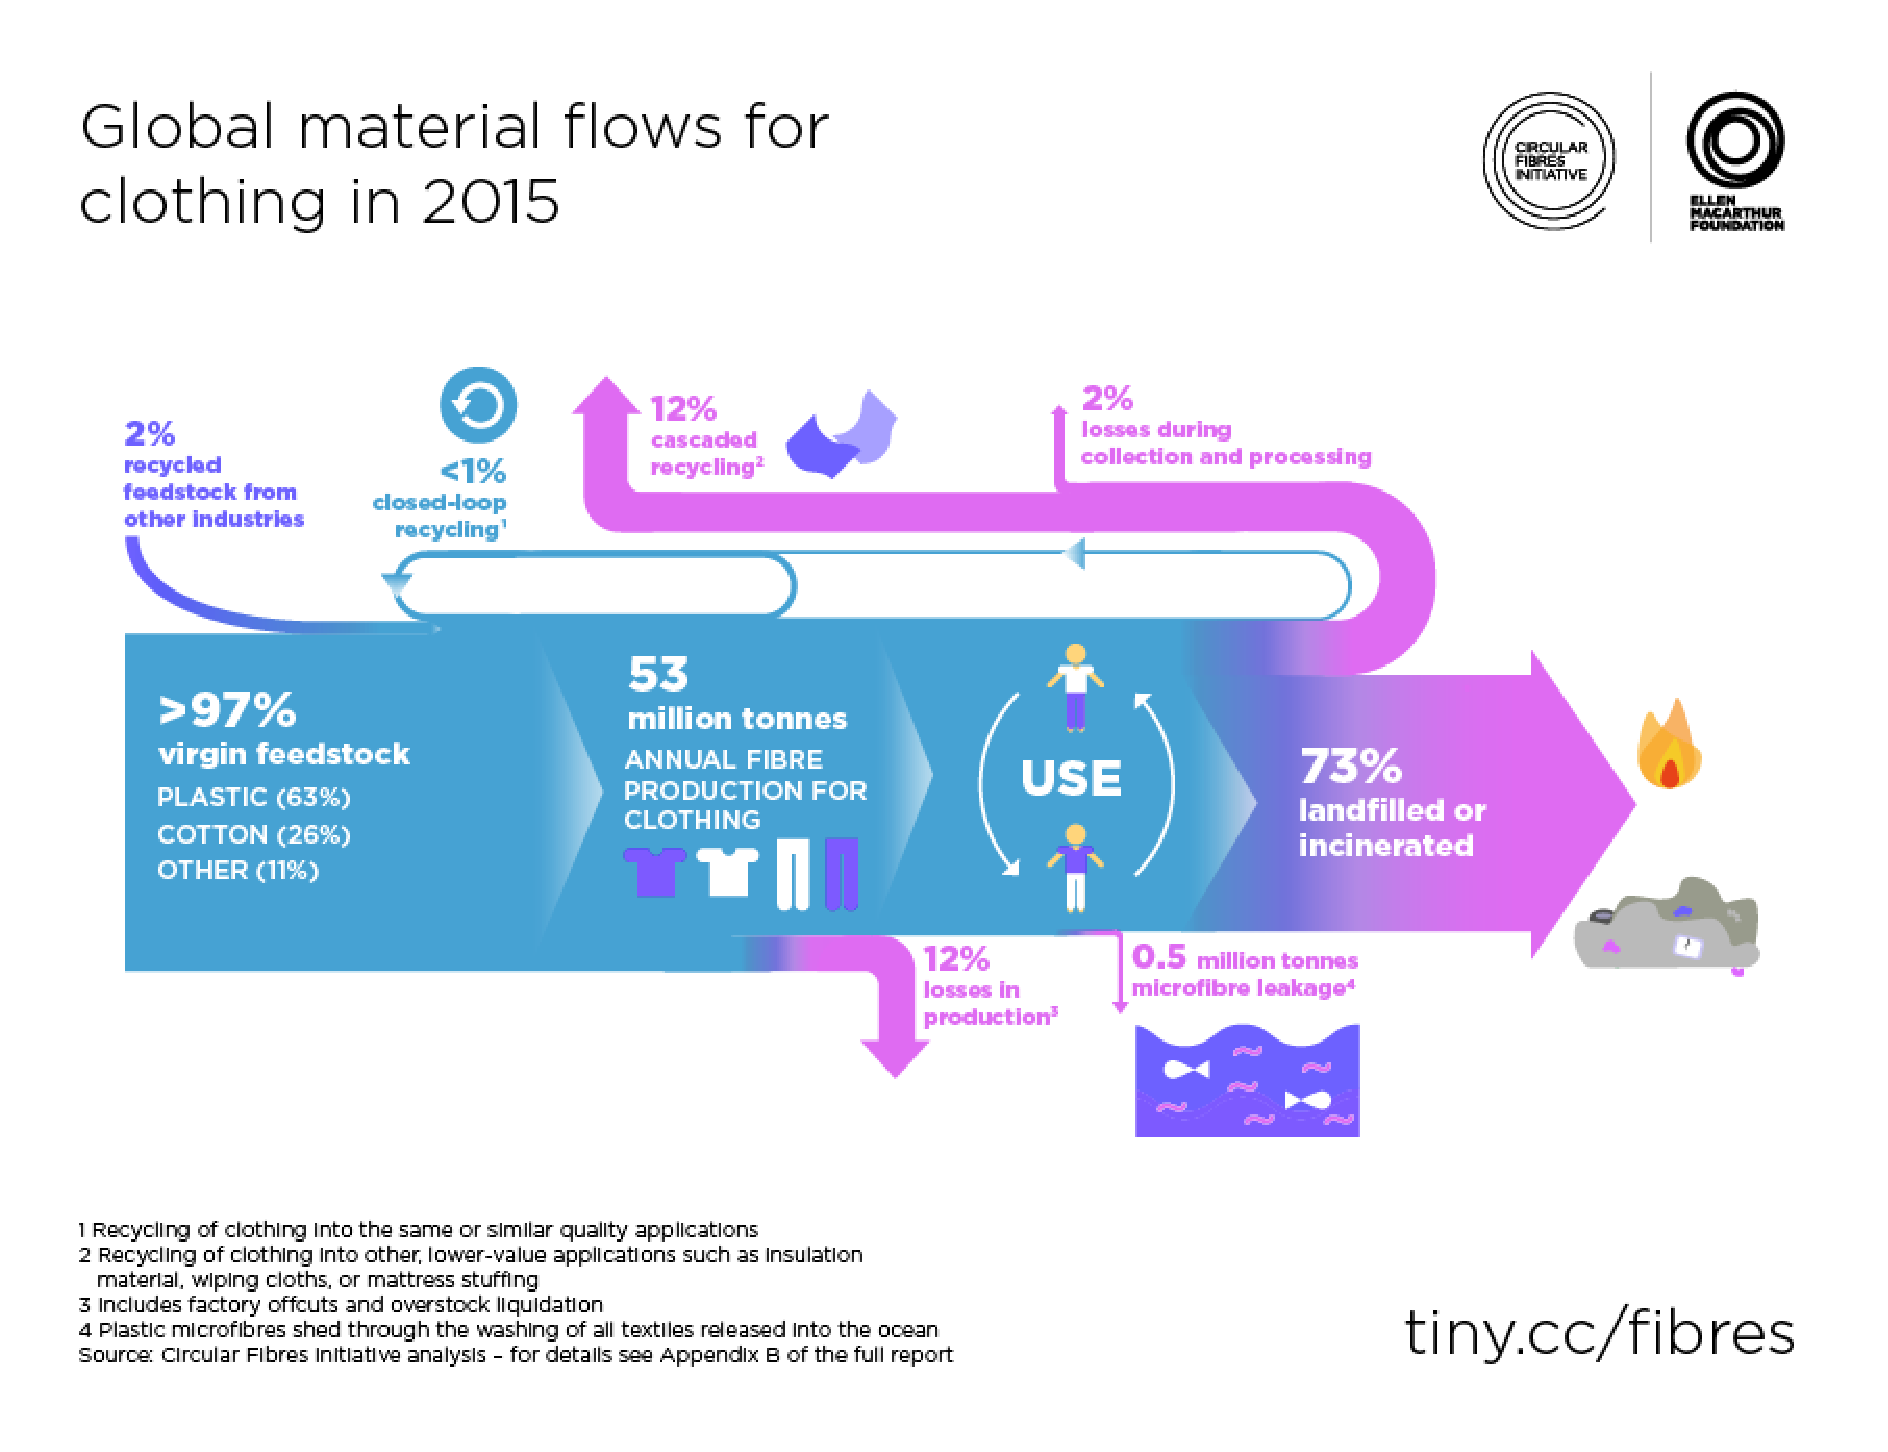
\includegraphics[width=0.7\textwidth]{figures/Figure-3_-Global-material-flows-for-clothing-in-2015.pdf}
 \caption{Infographic for the global material flows for clothing industry (adapted from \citep{Morlet2017}) }\label{fig:MaterialFlow}
 \end{center}
\end{figure}

Apart from technological advances in new, better, environmentally-friendly alternative fibers and dyes \citep{A.R.Bunsell2018,Shahid2013} or better recycling technologies \citep{Woolridge2006}, more sustainable business models can help in reducing the environmental impact of clothes by prolonging the clothes' lifetime. \citep{Elander2017} distinguish business models that (1) allow sharing clothes with others such as leasing of clothing libraries \citep{Pedersen2015,Zamani2017}, (2) collect used garments and resell them \citep{Farrant2010}, (3) extend the technical lifetime through better product design , and (5) redesign unsold or used textile products into a new product. These business models can only be economically viable if consumers are willing to participate and/or pay for these (often labor-expensive) collecting, sorting, repair, and laundering activities. This survey aims to inform companies about the market potential of these new business models and may help policy makers in choosing the right incentives to help these businesses \citep{Watson2017}.

This study focuses on 16-to-35-year-olds (also called \emph{millennials} or \emph{Generation Y}) and analyses their clothes consumptions patterns, what they are looking for in clothing and what they are willing to pay for. These people are the consumers of the future and previous studies have shown that, although they are more environmentally conscious, they are reluctant to change their consumptions patterns. This study should yield insights into whether these consumers are open to the previously mentionned new business models and ideas and whether they are willing to pay extra for sustainable clothing.

\cite{Farsang2014} describe the results of a similar study on clothing and fashion consumption by millennials in  Germany, the Netherlands, Sweden, the UK and the US. Their dataset had over 6000 respondents but their analysis was largely explorative; no deeper analysis with regression models or significance tests were performed.

\section{Method and data collection}\label{sec:method}
This section elaborates on the chosen focus group for our study (Section~\ref{subsec:method-data}) and on how the Discrete-choice experiment was designed (Section~\ref{subsec:method-dce}).

\subsection{Population and data development}\label{subsec:method-data}
Our study focuses on people between 15 and 35 years old that are living in Brussels or Flanders (Belgium). The questionnaire was developed in cooperation with second Bachelor students, based on previous research and their own experience. 

We question the respondents about socio-demographic characteristics, shopping and fashion preferences, their preferences for buying a T-shirt in a disrecte choice experiment, and their general attitudes towards sustainability, ecolabels, and use of sustainable business models. 

\subsection{Discrete choice experiment}\label{subsec:method-dce}
In the stated choice experiment, respondents were asked to choose between two T-shirts, labeled `A' and `B', and an opt-out option (\emph{`Neither of these'}). Based on brainstorm sessions and previous surveys on sustainable fashion (see literature review in Section~\ref{sec:Intro}), six attributes were used to describe the alternatives (see Table~\ref{tab:attributes}). It was explicitly stated that the T-shirt had to be paid with their own money, and that both T-shirts are short-sleeved, in their favorite color, and with their favorite neckline. 

\begin{table}[ht]
\begin{center}
\begin{tabular}{l l:ll }
\hline
Attribute & Attribute levels&Attribute & Attribute levels\\
\hline
Type of fibre&New cotton&Durability&Short life\\
&Recycled cotton&&Long life\\\cline{3-4}
&New polyester&Brand & Generic\\
&Recycled polyester&&Designer\\\hline
Label&Ecolabel&Country of &European Union\\
&No label&manufacturing&Asia\\\hline
Use&New&Price per T-shirt & 7 - 10 - 14 -\\
&Previously used (2$^{nd}$ hand)&(euro)&19 - 24 - 32\\
\hline
\end{tabular}
\caption{Attributes and attribute levels}
\label{tab:attributes}
\end{center}
\end{table}

To keep the number of choices for each respondent manageable, a D-efficient design with fixed priors and expected signs of two blocks with each six choice cards consisting of two unlabeled profiles and opt-out was determined in Ngene (a ChoiceMetrics software \citep{ChoiceMetrics}).

The data are first analyzed by a conditional logit (CL) model which assumes a linear relationship between utility and attribute parameters and thus requires the error term to be identically and independently distributes according to a Weibull distribution \citep{Mariel2013}. Next, a latent-class model is fitted which includes socio-economic and attitude variables heterogeneity in the respondent's preferences. All analysis was done using the \emph{gmnl} package for R \citep{sarrias2017multinomial}.

\section{Description of the dataset}\label{sec:data}
In total, there are \gls{demN} respondents between 16 and 35 years old. Only respondents living in Flanders or Brussels were kept for analysis.  \gls{demfemale}\% of respondents are female while \gls{demmale}\% are male. The imbalance in the gender-distribution is likely related to the topic of the study which appeals more to female shoppers.

Figure~\ref{fig:DemAgeGender} shows that many respondents are between 21 and 25 years old. This is not surprising as the survey was part of a course that was taught to third bachelor students who were asked to spread the survey. This is also reflected in the job and financial situation of the respondents (Figure~\ref{fig:JobIncome}); over half of them are students and only a minority (\gls{struggling}\%) indicate that they are financially struggling to make ends meet.

\begin{figure}[ht]
\begin{center}
 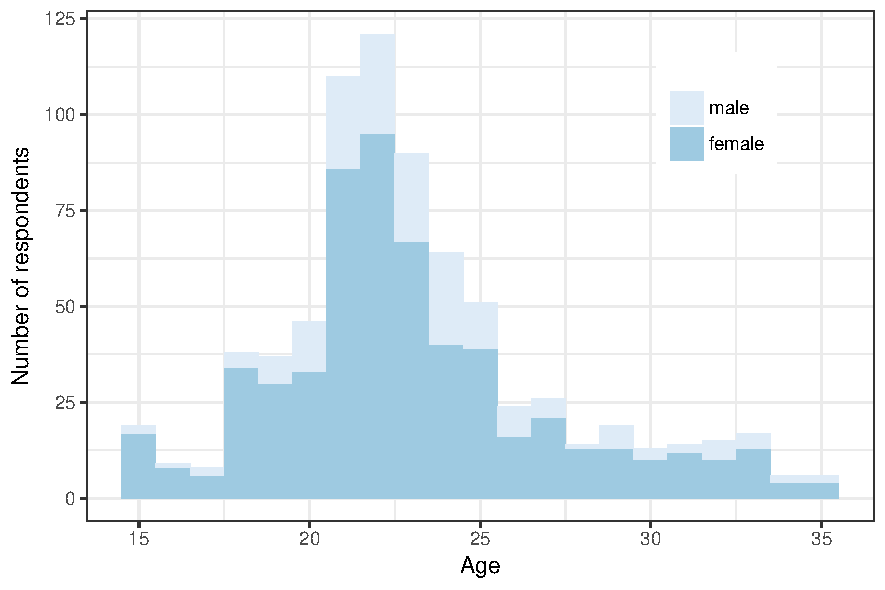
\includegraphics[width=0.7\textwidth]{figures/DemAgeGender.pdf}
 \caption{Age and gender distributions of the respondents}\label{fig:DemAgeGender}
 \end{center}
\end{figure}
\begin{figure}[ht]
\begin{center}
 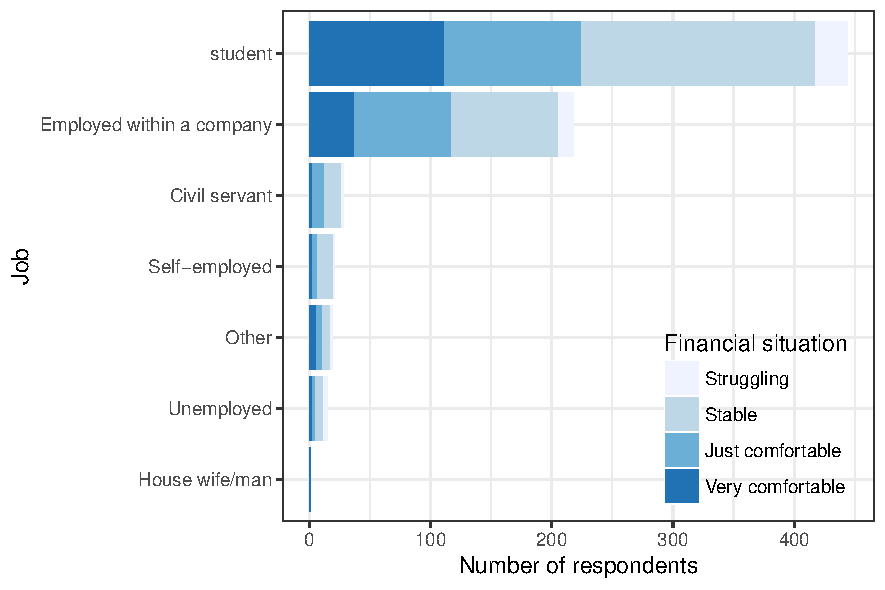
\includegraphics[width=0.7\textwidth]{figures/DemJobIncome.pdf}
 \caption{Job and financial situation of the respondents}\label{fig:JobIncome}
 \end{center}
\end{figure}

\subsection{shopping behavior}
Next to demographics, we also questioned respondents about their typical shopping behavior (Figure~\ref{fig:ShopLoc}) and which features they find important when buying clothes (Figure~\ref{fig:ShopClothing}). The high streets are the most popular shopping location but on-line shopping is equally popular for frequent shoppers (those who shopped more than 5 times in two months). Swapping and second hand markets offer consumers an opportunity to extent the lifetime of clothes but they are far less popular. Price, comfort, and fit (Figure~\ref{fig:ShopClothing}). 

\begin{figure}[ht]
\begin{center}
 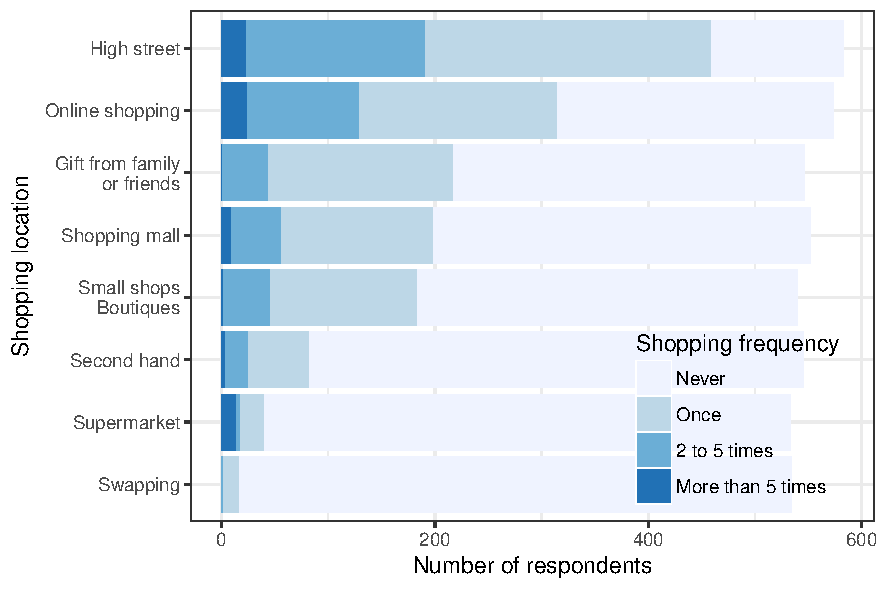
\includegraphics[width=0.7\textwidth]{figures/ShopLoc.pdf}
\caption{Response when asked where and how often they went shopping in January or February 2018}\label{fig:ShopLoc}
 \end{center}
\end{figure}
\begin{figure}[ht]
\begin{center}
 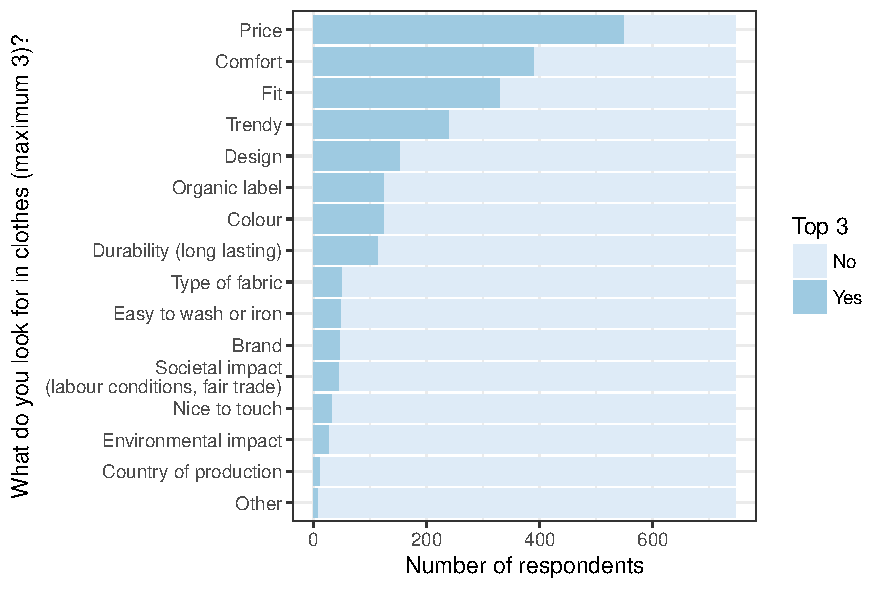
\includegraphics[width=0.7\textwidth]{figures/ShopClothing.pdf}
 \caption{Clothing features considered to be important (up to 3 characteristics would be selected by each respondent)}\label{fig:ShopClothing}
 \end{center}
\end{figure}

\subsection{Consumer attitudes}
The survey ended with some questions regarding environmental attitudes and shopping habits. Figure~\ref{fig:Attitudes1} shows that trendy and durable clothing is particularly important. Most respondents don't really seem to care whether their clothing has and ecolabel and few appreciate second-hand clothes or low maintenance fibers.  

\begin{figure}[ht]
\begin{center}
 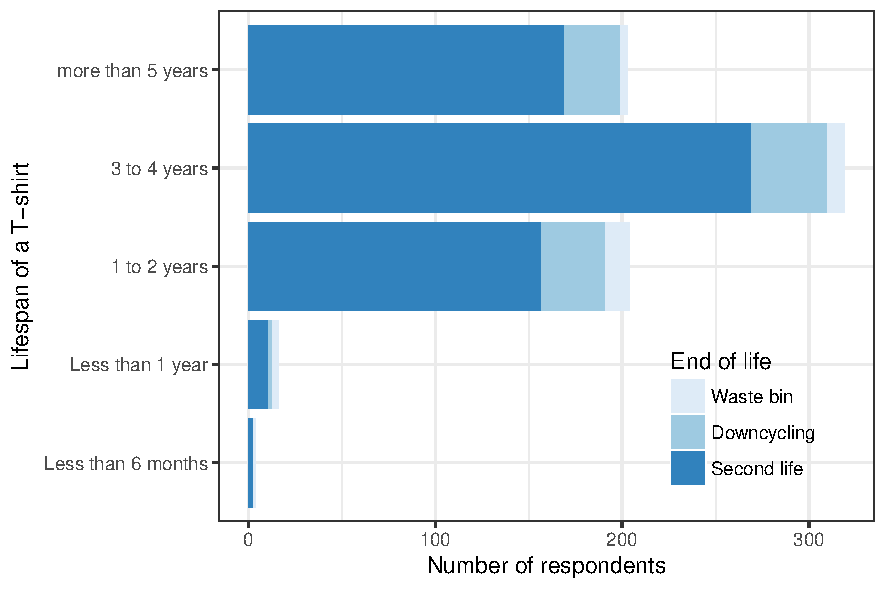
\includegraphics[width=0.95\textwidth]{figures/EndOfLife.pdf}
 \caption{Environmental attitude and shopping behavior.}\label{fig:EndOfLife}
 \end{center}
\end{figure}
\begin{figure}[ht]
\begin{center}
 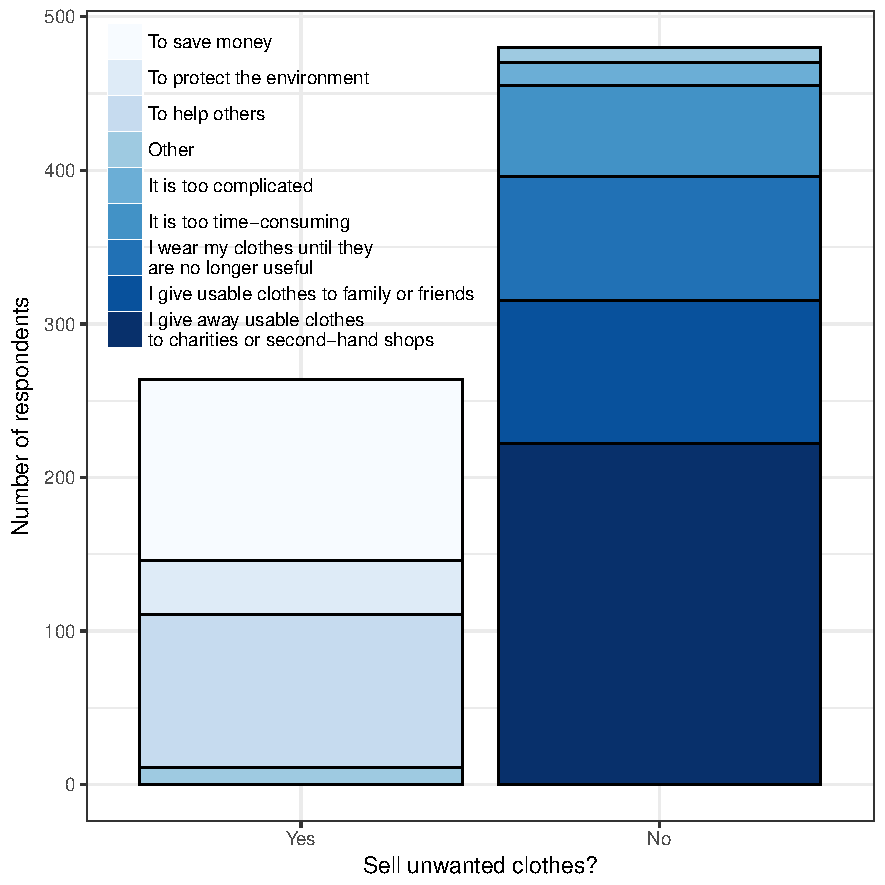
\includegraphics[width=0.95\textwidth]{figures/Sell2ndhand.pdf}
 \caption{Current use of repair services and novel business models.}\label{fig:Sell2ndhand}
 \end{center}
\end{figure}

\subsection{Clothing end of use}



\begin{figure}[ht]
\begin{center}
 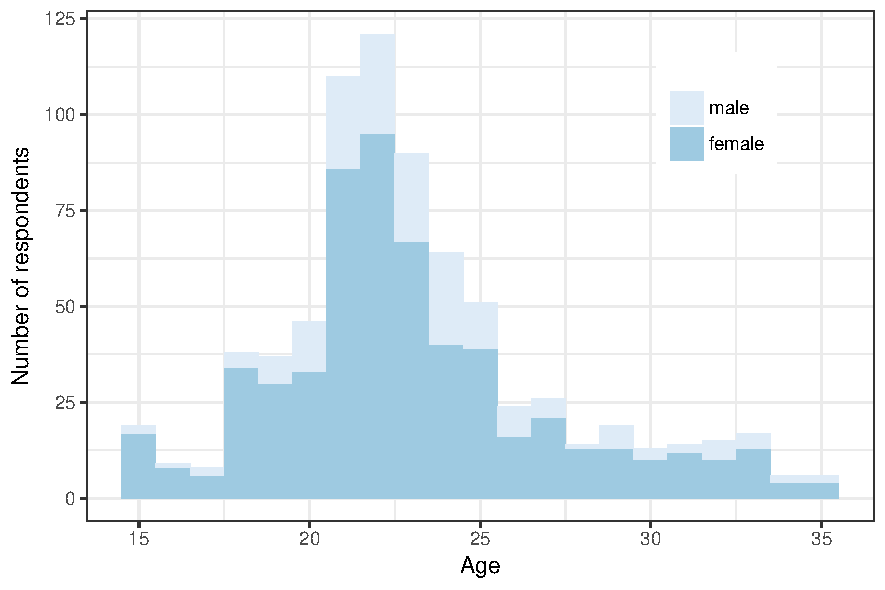
\includegraphics[width=0.7\textwidth]{figures/DemAgeGender.pdf}
 \caption{Age and gender distributions of the respondents}\label{fig:DemAgeGender}
 \end{center}
\end{figure}
\begin{figure}[ht]
\begin{center}
 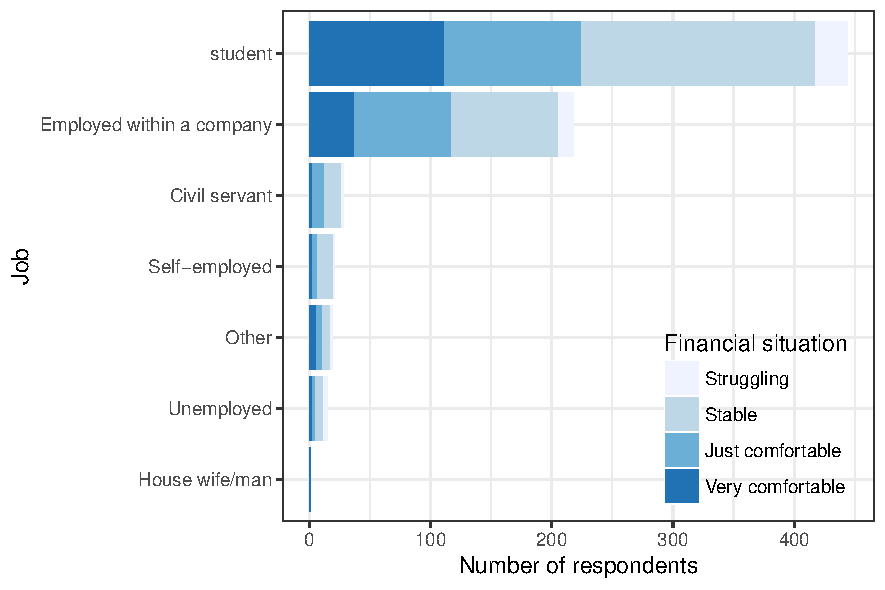
\includegraphics[width=0.7\textwidth]{figures/DemJobIncome.pdf}
 \caption{Job and financial situation of the respondents}\label{fig:JobIncome}
 \end{center}
\end{figure}

\section{Estimation results}\label{sec:results}
The conditional logit model of Table~\ref{tab:ConditionalLogitModel} shows that all variables are significant at the 5\% level. The coefficients can be transformed into WTP estimates which are shown in Table~\ref{tab:ConditionalLogitModelWTP}.


\begin{table}[ht]
\begin{center}
\begin{tabular}{l c }
\hline
 & Conditional logit model,\\ & coefficient and standard errors \\
\hline
cottonnew   & $0.424 \; (0.077)^{***}$  \\
cottonrec   & $0.335 \; (0.072)^{***}$  \\
polyrec     & $0.163 \; (0.070)^{*}$    \\
new         & $1.247 \; (0.068)^{***}$  \\
designer    & $0.261 \; (0.042)^{***}$  \\
ecolabel    & $0.293 \; (0.041)^{***}$  \\
eu          & $0.310 \; (0.041)^{***}$  \\
longuse     & $0.650 \; (0.055)^{***}$  \\
price       & $-0.063 \; (0.006)^{***}$ \\
ASC1        & $0.764 \; (0.166)^{***}$  \\
ASC2        & $0.738 \; (0.163)^{***}$  \\
\hline
AIC         & 7245.206                  \\
R$^2$       & 0.177                     \\
Max. R$^2$  & 0.519                     \\
Num. events & 4482                      \\
Num. obs.   & 13446                     \\
Missings    & 0                         \\
\hline
\multicolumn{2}{l}{\scriptsize{$^{***}p<0.001$, $^{**}p<0.01$, $^*p<0.05$}}
\end{tabular}
\caption{Conditional logit results}
\label{tab:ConditionalLogitModel}
\end{center}
\end{table}

% latex table generated in R 3.4.2 by xtable 1.8-2 package
% Tue Apr 17 11:05:17 2018
\begin{table}[ht]
\centering
\begin{tabular}{lccc}
  \hline
 & Mean WTP (euros per T-shirt) & Lower limit (2.5\%) & Upper limit (97.5\%) \\ 
  \hline
cottonnew & 6.78 & 4.11 & 9.45 \\ 
  cottonrec & 5.36 & 2.92 & 7.79 \\ 
  polyrec & 2.61 & 0.33 & 4.89 \\ 
  new & 19.96 & 15.79 & 24.12 \\ 
  designer & 4.17 & 2.64 & 5.71 \\ 
  ecolabel & 4.69 & 3.25 & 6.13 \\ 
  eu & 4.96 & 3.43 & 6.50 \\ 
  longuse & 10.40 & 8.08 & 12.72 \\ 
  ASC1 & 12.23 & 8.09 & 16.37 \\ 
  ASC2 & 11.80 & 7.69 & 15.92 \\ 
   \hline
\end{tabular}
\caption{mean WTP with confidence intervals for the conditional logit model} 
\label{tab:ConditionalLogitModelWTP}
\end{table}

% latex table generated in R 3.4.2 by xtable 1.8-2 package
% Tue Apr 17 11:05:17 2018
\begin{table}[ht]
\centering
\begin{tabular}{lccc}
  \hline
 & coefficient & p-value & WTP (euro) \\ 
  \hline
cottonnew & 0.424 & 3.076E-08 & 6.784 \\ 
  cottonrec & 0.335 & 3.124E-06 & 5.359 \\ 
  polyrec & 0.163 & 2.022E-02 & 2.610 \\ 
  new & 1.247 & 0.000E+00 & 19.955 \\ 
  designer & 0.261 & 7.268E-10 & 4.173 \\ 
  ecolabel & 0.293 & 7.951E-13 & 4.686 \\ 
  eu & 0.310 & 3.153E-14 & 4.964 \\ 
  longuse & 0.650 & 0.000E+00 & 10.399 \\ 
  price & -0.063 & 0.000E+00 &  \\ 
  ASC1 & 0.764 & 4.036E-06 &  \\ 
  ASC2 & 0.738 & 6.149E-06 &  \\ 
   \hline
\end{tabular}
\caption{conditional logit results} 
\label{tab:ConditionalLogitModelsummary}
\end{table}

\begin{table}[ht]
\begin{center}
\begin{tabular}{l c }
\hline
 & Conditional logit model,\\ & coefficient and standard errors \\
\hline
cottonnew       & $0.413 \; (0.122)^{***}$  \\
intcotnewstud   & $0.033 \; (0.157)$        \\
cottonrec       & $0.242 \; (0.113)^{*}$    \\
intcotrecstud   & $0.166 \; (0.146)$        \\
polyrec         & $0.068 \; (0.114)$        \\
intpolyrecstud  & $0.165 \; (0.145)$        \\
new             & $1.362 \; (0.114)^{***}$  \\
intnewstud      & $-0.183 \; (0.142)$       \\
designer        & $0.159 \; (0.066)^{*}$    \\
intdesignerstud & $0.171 \; (0.086)^{*}$    \\
ecolabel        & $0.231 \; (0.065)^{***}$  \\
intecostud      & $0.105 \; (0.083)$        \\
eu              & $0.313 \; (0.065)^{***}$  \\
inteustud       & $-0.002 \; (0.084)$       \\
longuse         & $0.668 \; (0.087)^{***}$  \\
intlongstud     & $-0.026 \; (0.112)$       \\
price           & $-0.063 \; (0.006)^{***}$ \\
ASC1            & $0.835 \; (0.235)^{***}$  \\
intasc1stud     & $-0.138 \; (0.266)$       \\
ASC2            & $0.849 \; (0.230)^{***}$  \\
intasc2stud     & $-0.204 \; (0.264)$       \\
\hline
AIC             & 7248.687                  \\
R$^2$           & 0.178                     \\
Max. R$^2$      & 0.519                     \\
Num. events     & 4482                      \\
Num. obs.       & 13446                     \\
Missings        & 0                         \\
\hline
\multicolumn{2}{l}{\scriptsize{$^{***}p<0.001$, $^{**}p<0.01$, $^*p<0.05$}}
\end{tabular}
\caption{Conditional logit results with student interaction effect}
\label{tab:ConditionalLogitModelStud}
\end{center}
\end{table}

\begin{table}[ht]
\begin{center}
\begin{tabular}{l c }
\hline
 & Conditional logit model,\\ & coefficient and standard errors \\
\hline
cottonnew      & $0.343 \; (0.111)^{**}$   \\
intcotnewtex   & $0.192 \; (0.155)$        \\
cottonrec      & $0.217 \; (0.101)^{*}$    \\
intcotrectex   & $0.292 \; (0.146)^{*}$    \\
polyrec        & $0.030 \; (0.099)$        \\
intpolyrectex  & $0.308 \; (0.142)^{*}$    \\
new            & $1.575 \; (0.093)^{***}$  \\
intnewtex      & $-0.741 \; (0.135)^{***}$ \\
designer       & $0.420 \; (0.059)^{***}$  \\
intdesignertex & $-0.370 \; (0.086)^{***}$ \\
ecolabel       & $0.231 \; (0.058)^{***}$  \\
intecotex      & $0.178 \; (0.082)^{*}$    \\
eu             & $0.318 \; (0.055)^{***}$  \\
inteutex       & $0.008 \; (0.082)$        \\
longuse        & $0.709 \; (0.078)^{***}$  \\
intlongtex     & $-0.111 \; (0.108)$       \\
price          & $-0.064 \; (0.006)^{***}$ \\
ASC1           & $0.562 \; (0.204)^{**}$   \\
intasc1tex     & $0.430 \; (0.256)$        \\
ASC2           & $0.556 \; (0.199)^{**}$   \\
intasc2tex     & $0.369 \; (0.255)$        \\
\hline
AIC            & 7162.421                  \\
R$^2$          & 0.184                     \\
Max. R$^2$     & 0.519                     \\
Num. events    & 4482                      \\
Num. obs.      & 13446                     \\
Missings       & 0                         \\
\hline
\multicolumn{2}{l}{\scriptsize{$^{***}p<0.001$, $^{**}p<0.01$, $^*p<0.05$}}
\end{tabular}
\caption{Conditional logit results with labelled textile buyer interaction effect}
\label{tab:ConditionalLogitModelBlt}
\end{center}
\end{table}

% latex table generated in R 3.4.2 by xtable 1.8-2 package
% Tue Apr 17 11:05:31 2018
\begin{table}[ht]
\centering
\begin{tabular}{lcccccc}
  \hline
 & coef1 & pvalue1 & coef2 & pvalue2 & coef3 & pvalue3 \\ 
  \hline
cottonnew & 0.252 & 0.057 & 0.770 & 0.000 & 2.278 & 0.019 \\ 
  cottonrec & 0.148 & 0.179 & 0.490 & 0.014 & 1.341 & 0.004 \\ 
  polyrec & 0.165 & 0.185 & 0.247 & 0.228 & 0.747 & 0.073 \\ 
  new & 0.588 & 0.000 & 0.650 & 0.000 & 3.678 & 0.000 \\ 
  designer & 0.332 & 0.000 & -0.169 & 0.150 & 0.599 & 0.000 \\ 
  ecolabel & 0.461 & 0.000 & 0.241 & 0.037 & -0.087 & 0.675 \\ 
  eu & 0.630 & 0.000 & 0.496 & 0.000 & -0.023 & 0.927 \\ 
  longuse & 0.998 & 0.000 & 0.569 & 0.000 & 0.576 & 0.116 \\ 
  price & 0.058 & 0.003 & -0.105 & 0.000 & -0.140 & 0.000 \\ 
  ASC1 & -0.318 & 0.376 & 0.280 & 0.405 & 1.139 & 0.252 \\ 
  ASC2 & -0.367 & 0.306 & 0.111 & 0.737 & 1.558 & 0.073 \\ 
  Class & 0.000 & 0.000 & -0.710 & 0.000 & 0.184 & 0.000 \\ 
  Class share & 0.371 & 0.000 & 0.182 & 0.000 & 0.446 & 0.000 \\ 
   \hline
\end{tabular}
\caption{coefficient estimates and p-values for each class} 
\label{tab:Latentclasses1}
\end{table}

\begin{figure}[ht]
\begin{center}
 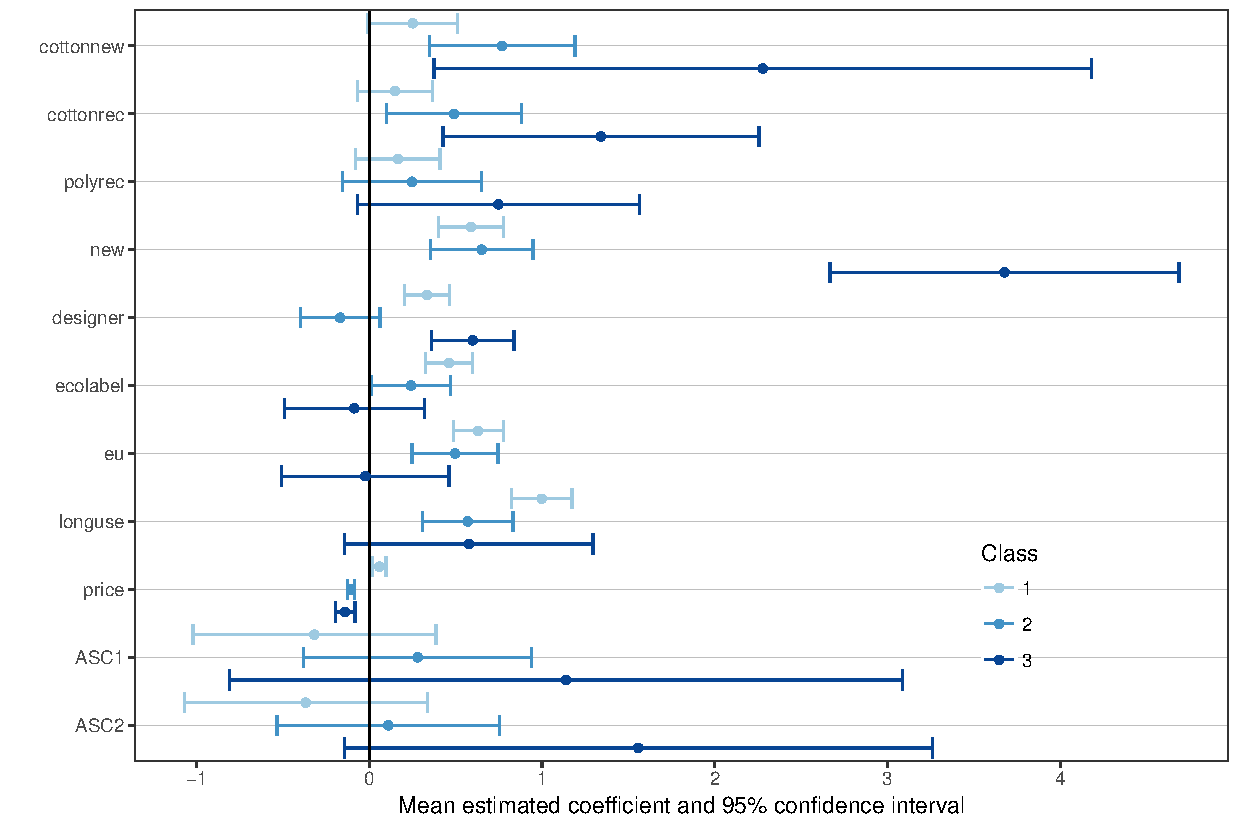
\includegraphics[width=0.95\textwidth]{figures/LatentClasses.pdf}
 \caption{Results for a conditional logit model with three latent classes}\label{fig:Habits}
 \end{center}
\end{figure}

\section{Discussion}\label{sec:discussion}

\section{Conclusion}\label{sec:conclusion}



\section*{References}

\bibliography{mybibfile}

\end{document}